\documentclass[tikz, border=10pt]{standalone}

\usepackage{amssymb}
\usepackage{amsmath}

\usepackage{tikz}
\usetikzlibrary{
    positioning,
    arrows.meta,
    shapes.geometric,
    calc
}

\begin{document}

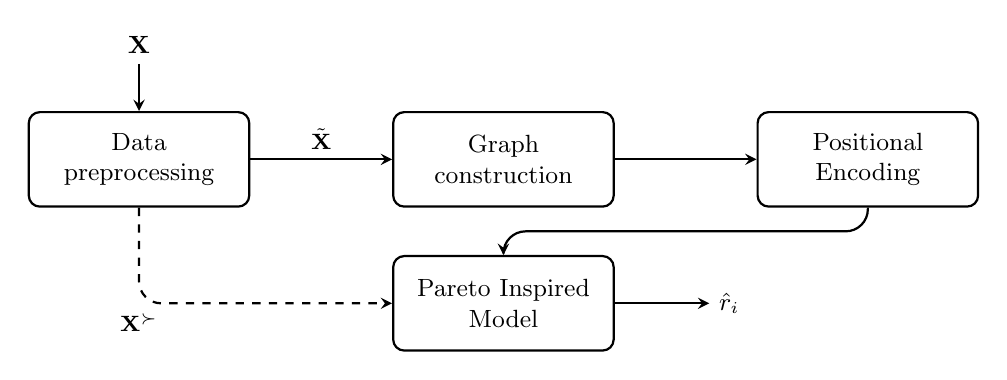
\begin{tikzpicture}[
    every node/.style={font=\small},
    block/.style={
        rectangle,
        draw,
        rounded corners=4pt,
        align=center,
        minimum height=1.2cm,
        minimum width=2.8cm,
        thick
    },
    arrow/.style={->, thick, >=stealth},
    label/.style={font=\footnotesize, midway, above}
]

% ---------- Nodes (left to right) ----------
\node (X) {$\mathbf{X}$};

\node[block, below=0.6cm of X] (pre) {Data\\preprocessing};

\node[block, right=1.8cm of pre] (graph) {Graph\\construction};

\node[block, right=1.8cm of graph] (pos) {Positional\\Encoding};

\node[block, below=0.6cm of graph] (model) {Pareto Inspired \\ Model};

\node[right=1.2cm of model] (s) {$\hat{r}_i$};

% ---------- Main pipeline arrows ----------
\draw[arrow] (X)     -- (pre);
\draw[arrow] (pre)   -- node[label] {$\tilde{\mathbf{X}}$} (graph);
\draw[arrow] (graph) -- (pos);
% \draw[arrow] (pos)   -- (model);
\draw[arrow] (model) -- (s);

% ---------- Dashed bypass arrow (pre → model, below) ----------
\draw[arrow, dashed, rounded corners=8pt]
    (pre.south)
    |- node[font=\footnotesize, pos=0.5, below]
    {$\mathbf{X}^\succ$}
    (model.west);

\draw[arrow, rounded corners=8pt]
    (pos.south)
    -- ++(0, -0.3) -|
    (model.north);

\end{tikzpicture}

\end{document}
